\documentclass[11pt]{article}
\usepackage[utf8]{inputenc}
%\usepackage[latin1]{inputenc}
\usepackage[spanish]{babel}
\decimalpoint
\usepackage{anysize}
\usepackage{graphicx} 
\usepackage{amsmath}
\usepackage{booktabs}
\usepackage{tabulary}
\usepackage{nccmath}
\usepackage{float}
\usepackage{tikz}
\usetikzlibrary{patterns}
\usetikzlibrary{decorations.markings}
\usepackage{pgfplots}
\usepackage{etex}
\usepackage{color}
\usepackage{listings}
\renewcommand{\arraystretch}{1.5}
\lstset{ %
language=Python,                % choose the language of the code
basicstyle=\normalsize,       % the size of the fonts that are used for the code
numbers=left,                   % where to put the line-numbers
numberstyle=\footnotesize,      % the size of the fonts that are used for the line-numbers
stepnumber=1,                   % the step between two line-numbers. If it is 1 each line will be numbered
numbersep=5pt,                  % how far the line-numbers are from the code
backgroundcolor=\color{white},  % choose the background color. You must add \usepackage{color}
showspaces=false,               % show spaces adding particular underscores
showstringspaces=false,         % underline spaces within strings
showtabs=false,                 % show tabs within strings adding particular underscores
frame=single,   		% adds a frame around the code
tabsize=4,  		% sets default tabsize to 2 spaces
captionpos=b,   		% sets the caption-position to bottom
breaklines=true,    	% sets automatic line breaking
breakatwhitespace=false,    % sets if automatic breaks should only happen at whitespace
escapeinside={\#}{)}          % if you want to add a comment within your code
}
\marginsize{1.5cm}{1.5cm}{-1cm}{1cm}  
\title{Tarea Integración \\ Curso de Física Computacional}
\author{M. en C. Gustavo Contreras Mayén}
\date{ }
\begin{document}
\maketitle
\fontsize{14}{14}\selectfont
\begin{enumerate}
\item Usa la regla del trapecio recursiva para evaluar
\[ \int_{0}^{\frac{\pi}{4}} ln(1 + \tan(x)) dx\]
Explica tus resultados.
\item La siguiente tabla indica la potencia $P$ propocionada por las ruedas de un carro como función de la velocidad $v$. Si la masa del carro es $m=2000$ kg, calcula el tiempo $\Delta t$ necesario para que el carro acelere de $1$ m/s a $6$ m/s. Usa la regla del trapecio para integrar. Tip:
\[ \Delta t = m \int_{1s}^{6s} \left( \dfrac{v}{P} \right) dv\]
que se puede obtener de la ley de Newton $F= m/(dv/dt)$ y por la definición de potencia, $P=Fv$.
\begin{center}
\begin{tabular}{c | c | c | c | c | c | c | c | c}
$v$ (m/s) & 0 & 1.0 & 1.8 & 2.4 & 3.5 & 4.4 & 5.1 & 6.0 \\ \hline
$P$ (kW)  & 0 & 4.7 & 12.2 & 19.0 & 31.8 & 40.1 & 43.8 & 43.2 
\end{tabular}
\end{center}
\item La siguiente tabla proporciona el empuje $F$ del arco como función del desplazamiento $x$. Si la cuerda tiene un desplazamiento de $0.5$ m, calcula la velocidad de una flecha de $0.075$ kg, cuando sale del arco. Tip: la energía cinética de la flecha es igual al trabajo hecho al estirar la cuerda, que es:
\[ m \dfrac{v^{2}}{2} = \int_{0}^{0.5m} F dx\]
\begin{center}
\begin{tabular}{c | c | c | c | c | c | c |}
$x$ (m) & 0.00 & 0.05 & 0.10 & 0.15 & 0.20 & 0.25  \\ \hline
$F$ (N)  & 0 & 37 & 71 & 104 & 134 & 161
\end{tabular}
\end{center}
\begin{center}
\begin{tabular}{c | c | c | c | c | c | }
$x$ (m) & 0.30 & 0.35 & 0.40 & 0.45 & 0.50 \\ \hline
$F$ (N)  & 185 & 207 & 225 & 239 & 250 
\end{tabular}
\end{center}
\begin{figure}[H]
	\centering
	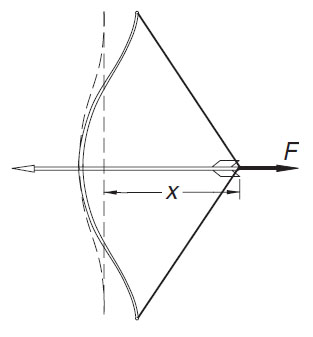
\includegraphics[scale=0.5]{Imagenes/Integral_01_Arco.jpg} 
	\caption{Flecha para el ejercicio}
\end{figure}
\item El período de un péndulo de longitud $L$ es $\tau = 4 \sqrt{\frac{L}{g}} h(\theta_{0})$, donde $g$ es la aceleración debida a la gravedad, $\theta_{0}$, representa la amplitud angular y 
\[ h(\theta_{0}) =  \int_{0}^{\frac{\pi}{2}} \dfrac{d\theta}{\sqrt{1 - \sin^{2} \left( \frac{\theta_{0}}{2}\right) \sin^{2} \theta}} \]
Calcular $h(15^{\circ})$, $h(30^{\circ})$ y $h(45^{\circ})$; compara esos valores con $h(0^{\circ}) = \frac{\pi}{2}$ (la aproximación usada para pequeñas amplitudes)
\item La fórmula de Debye para la capacidad calorífica $C_{v}$ de un sólido, es $C_{v} = 9 Nkg(u)$, donde
\[g(u) = u^{3} \int_{0}^{1/u} \dfrac{x^{4}e^{x}}{(e^{x}-1)}dx\]
los términos de la ecuación son:
\\
\\
\begin{minipage}{4cm}
\begin{eqnarray*}
N &=& \text{Número de partículas en el sólido} \\
k &=& \text{Constante de Boltzmann} \\
u &=& \frac{T}{\Theta_{D}}
\end{eqnarray*}
\end{minipage}
\hspace{3cm}
\begin{minipage}{4cm}
\begin{eqnarray*}
T &=& \text{temperatura absoluta} \\
\Theta_{D} &=& \text{Temperatura de Debye}
\end{eqnarray*}
\end{minipage}
\\
Calcular $g(u)$ para $u=0$ a $1.0$ en intervalos de $0.05$, grafica los resultados.
\item Una masa $m$ est\'{a} unida a un resorte de longitud $b$ y rigidez $k$. Se puede demostrar que la aceleración de la masa es $\ddot{x} = -f(x)$, donde
\[f(x) = \mu g + \dfrac{k}{m} (\mu b + x) \left( 1 - \dfrac{b}{\sqrt{b^{2} + x^{2}}} \right)\]
Si la masa se libera del reposo en $x=b$, y la velocidad en $x=0$ est\'{a} dada por
\[ v_{0} = \sqrt{2 \int_{0}^{b} f(x) dx}\]
\begin{figure}[H]
	\centering
	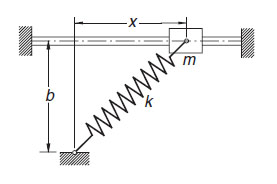
\includegraphics[scale=0.5]{Imagenes/Integral_02_Resorte.jpg}
	\caption{Masa unida a un resorte.}
\end{figure}
Calcular mediante integración numérica el valor de $v_{0}$, usando $m=0.8$ k, $b=0.4$ m, $\mu=0.3$, $k=80$ N/m y $g=9.81$ $m/s^{2}$.
\end{enumerate}
\end{document}